\chapter{How to Align}
\label{ch:howtoalign}

This chapter provides step-by-step instructions on how to align a new set of testbeam data without losing one's mind.

For the alignment of the telescope and DUT, these modules are available in \corry:
\begin{itemize}
\item \texttt{Prealignment} \textcolor{blue}{Jens: }\textcolor{orange}{I haven't ever used this really!}
\item \texttt{AlignmentTrackChi2} used for telescope alignment
\item \texttt{AlignmentDUTResidual} used for DUT alignment
\item \texttt{AlignmentMillipede} \textcolor{blue}{Jens: }\textcolor{orange}{I haven't ever used this really!}
\end{itemize}

Scripts to run and configure \corry should be stored in a separate git repository.
Working examples can be found here: \textbf{path/to/corryvreckan/testing/}.

It consists of two subdirectories (\textcolor{red}{not complete yet...will work on this}):
\begin{itemize}
\item \textbf{geometries/} contains all the detector files which provide detector information and alignment information
\item \textbf{configurations/} contains the scripts that are run to call and configure \corry for alignment and analysis.
\end{itemize}

\textbf{Note:} \corry can handle any file extensions for geometry and configuration files. The examples, however, follow the convention of using \texttt{*.geo} for geometry and \texttt{*.conf} for configuration files for clarity.

The general procedure that needs to be followed for a sucessful alignment is outlined here and explained in detail below.
\begin{enumerate}
\item prealign telescope (ignore DUT)
\item align telescope (ignore DUT)
\item prealign DUT (telescope geometry is frozen)
\item align DUT (telescope alignment is frozen)
\end{enumerate}

\section{Aligning the Telescope}
\label{sec:align_tel}
To begin with, the telescope needs to be aligned. 
For this, the DUT is completely ignored.

\subsection*{Prealignment of the Telescope}
The \texttt{AlignmentTrackChi2} module requires a careful prealignment. Otherwise it does not converge and the alignment will fail.
For the prealignment, two tricks can be played.
\begin{itemize}
\item A rough manual prealignment can be performed by having a look at correlations plots between a defined reference plane and the others planes in both x and y.
These can be found in the module \texttt{TestAlgorithm}.
\item The \texttt{Prealignment} module can be used.
\end{itemize}

Generally, the alignment file from the last testbeam is a solid basis to start from. Only the z-position of all planes (which need to be measured by hand in the setup) needs to be adjusted in the detectors file. 

\textbf{Note:} The z-position will not be changed during the alignment procedure.

To have a first look at the initial alignment guess, one can run
\begin{verbatim}
    /path/to/corryvreckan/bin/corry 
        -c analyse_telescope.conf
    	-o detectors_file=<detectorsFile> 
    	-o histogramFile=<histogramFile> 
    	-o EventLoaderTimepix3.inputDirectory=<inputDir>
\end{verbatim}

The \texttt{spatialCut} in \texttt{[Tracking4D]} should be set to mulitple ($\sim4$) pixel size.

Inspect the track $\chi^2$, the correlation in x and y and the residuals with the online monitoring or by opening the generated ROOT file after finishing the script (see \texttt{[Tracking4D]} and \texttt{[TestAlgorithm]}).

\textbf{Tip:} Terminate \corry with \texttt{Ctrl+C} after a while to save time.

If no peak at all is apparent in the correlations, something went terribly wrong.
In that case, have a look at the hitmaps to check if valid data is actually available for all planes.

For the residuals, zoom in and estimate the shift of the peak from 0 with a precision of $\mathcal{O}(\SI{100}{\micro m})$. 
For instance, if the peak is shifted by +\SI{+300}{\micro m} edit the detectors file and add \SI{+300}{\micro m} to the respective position, if \SI{-300}{\micro m}, subtract.
Then, run again until the peaks are roughly centered around 0.

\textbf{Note:} Don't force the peak of the \textit{correlations} to be at exactly 0 because the position of the peak in fact corresponds to the physical offset of the plane from its ideal position. What really needs to be centered around 0 are the \textit{residuals}.

As a next step, the \texttt{Prealignment} module can be run for an even better prealignment.\\
\textcolor{blue}{TODO: }\textcolor{orange}{I haven't ever used the [Prealignment] module, so maybe someone else can write a few sentences here.}

To do so, edit \texttt{align\_tel.conf} and make sure to enable the \texttt{Prealignment} and disable the \texttt{Alignment}:
\begin{minted}[frame=single,framesep=3pt,breaklines=true,tabsize=2,linenos]{ini}
...
[Prealignment]
[Ignore]
#[AlignmentTrackChi2]
log_level=INFO
iterations = 4
alignOrientation=true
alignPosition=true
\end{minted}

Then run
\begin{verbatim}
    /path/to/corryvreckan/bin/corry 
        -c align_telescope.conf
    	-o detectors_file=<detectorsFile> 
    	-o detectors_file_updated=<detectorsFileUpdated> 
    	-o histogramFile=<histogramFile> 
    	-o EventLoaderTimepix3.inputDirectory=<inputDir>
\end{verbatim}

The actual prealignment is only performed after the events have been analysed and written to the detectors file in the finalizing step. 
This means to check whether the alignment has improved, one needs to re-run the analysis or the next iteration of the alignment as the previously generated ROOT file corresponds to the alignment you started from.
This is the case for every iteration of the prealignment or alignment (\textbf{Don't forget this later!!}).

\subsection*{Alignment of the Telescope}
After the prealignment, the actual \textit{precise} alignment can be performed using the \texttt{AlignmentTrackChi2} module.
To this end, \texttt{align\_tel.conf} needs to be modified such that the prealignment is disabled and the alignment is enabled:
\begin{minted}[frame=single,framesep=3pt,breaklines=true,tabsize=2,linenos]{ini}
...
#[Prealignment]
#[Ignore]
[AlignmentTrackChi2]
log_level=INFO
iterations = 4
alignOrientation=true
alignPosition=true
\end{minted}

The algorithm performs an optimisation of the track $\chi^2$.
Typically, the alignment needs to be iterated a handful of times until the residuals (which again can be inspected in the ROOT file of the next iteration) are nicely centered around 0 and narrow.
In fact, the width of the residuals corresponds to the spatial resolution of each plane and should thus be smaller than the respective pixel size.
Starting with a \texttt{spatialCut} in \texttt{[Tracking4D]} of multiple ($\sim4$) pixel sizes, it should be decreased incrementally down to the pixel size (e.g. run \SI{200}{\micro\m} twice, then run \SI{150}{\micro\m} twice, then \SI{100}{\micro\m} twice, and then \SI{50}{\micro\m}) twice.
This allows to perform the alignment with a tight selection of very high quality tracks only.
Also the \texttt{max\_track\_chi2ndof} should be decrease for the same reason.
For the further analysis, the cut can be released again.

Sometimes, the procedure runs into a 'false minimum' or 'gets stuck' and does not converge properly which requires to go one step back and improve the prealignment.

Once the alignment is done, one should obtain narrow residuals centered around 0 and a good distribution of the track $\chi^2$ as shown in Figures~\ref{fig:exampleAlignment}.

If the alignment keeps to fail, it is possible to allow only for rotational or translational alignment while freezing the other for one or a few iterations.

\begin{figure}
    \centering
    \begin{subfigure}[t]{0.66\textwidth}
        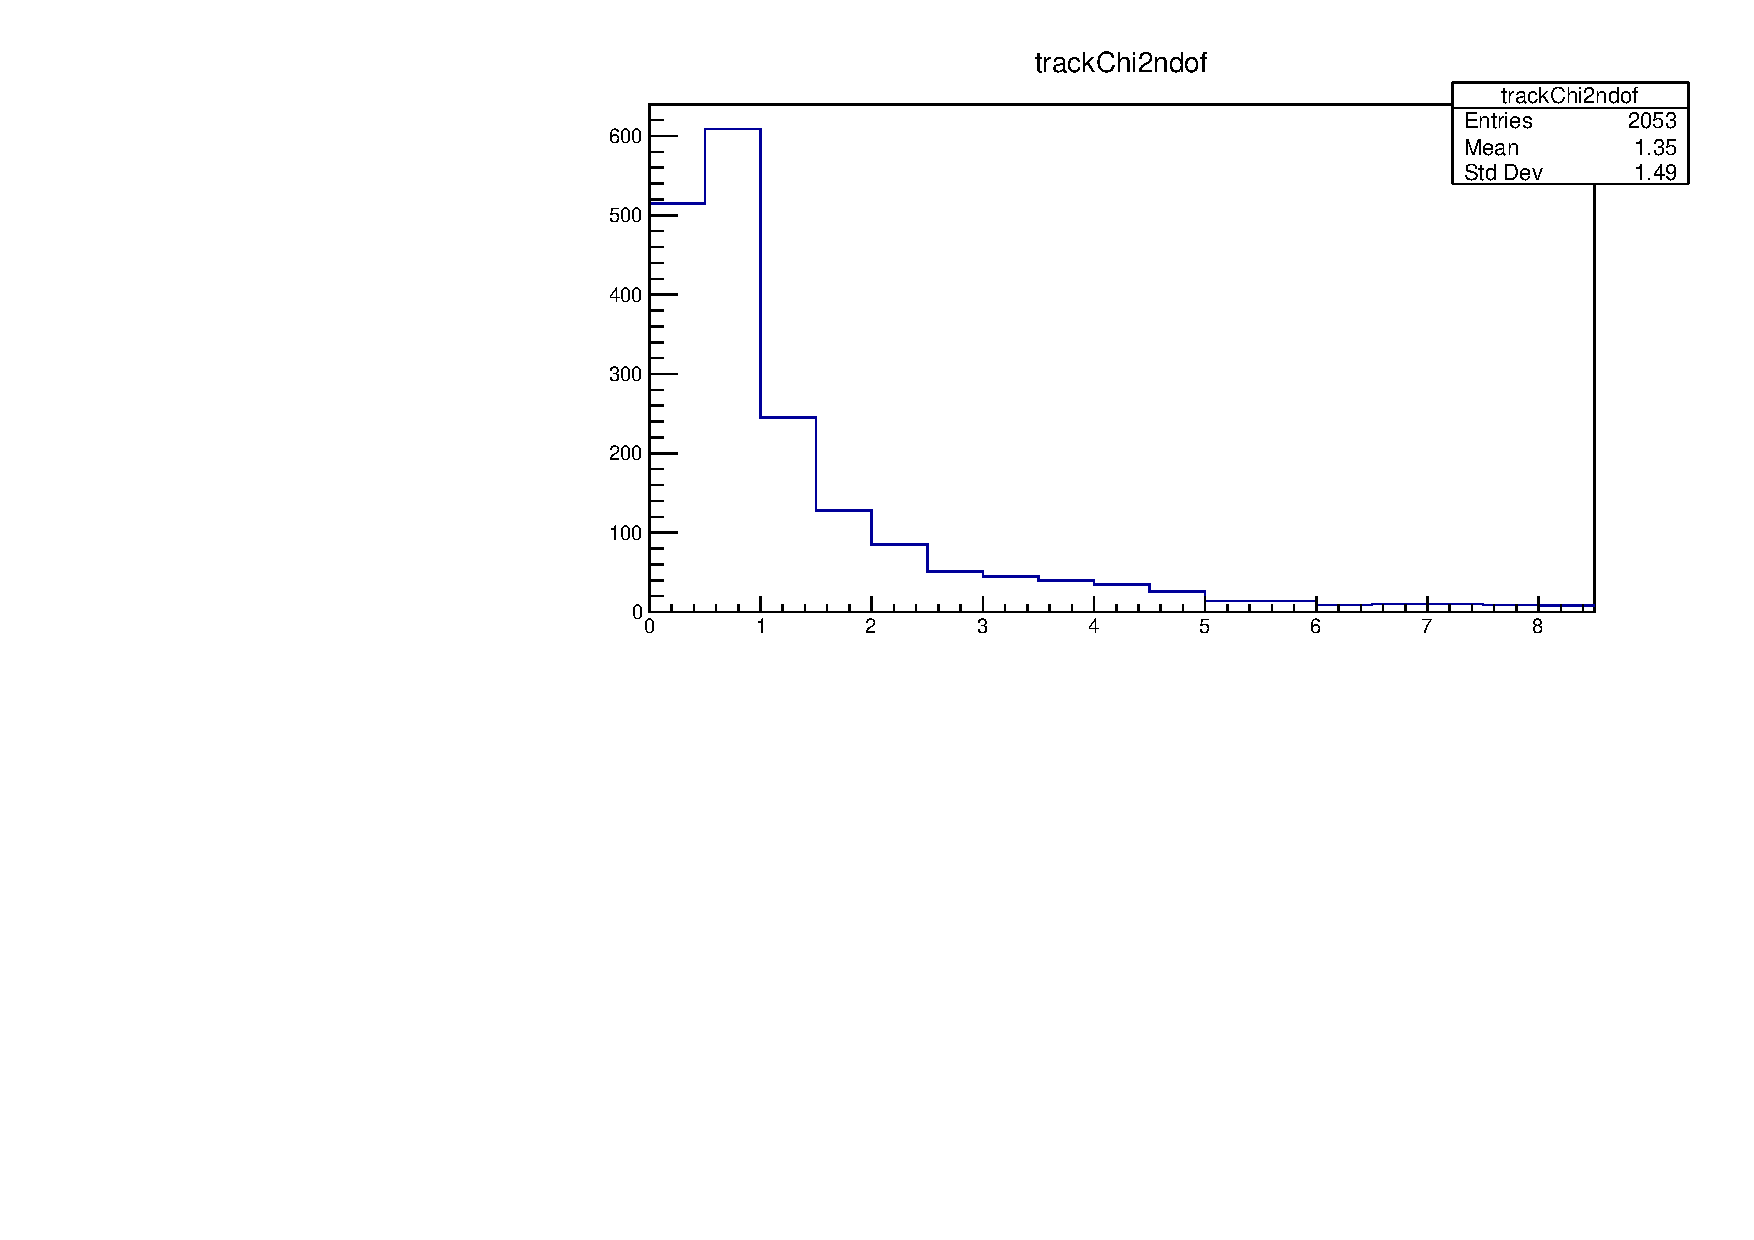
\includegraphics[width=\textwidth]{trackChi2_29519}
        \caption{Good example of a track $\chi^2$/ndf distribution.}
        \label{fig:trackChi2}
    \end{subfigure}
    \begin{subfigure}[t]{0.66\textwidth}
        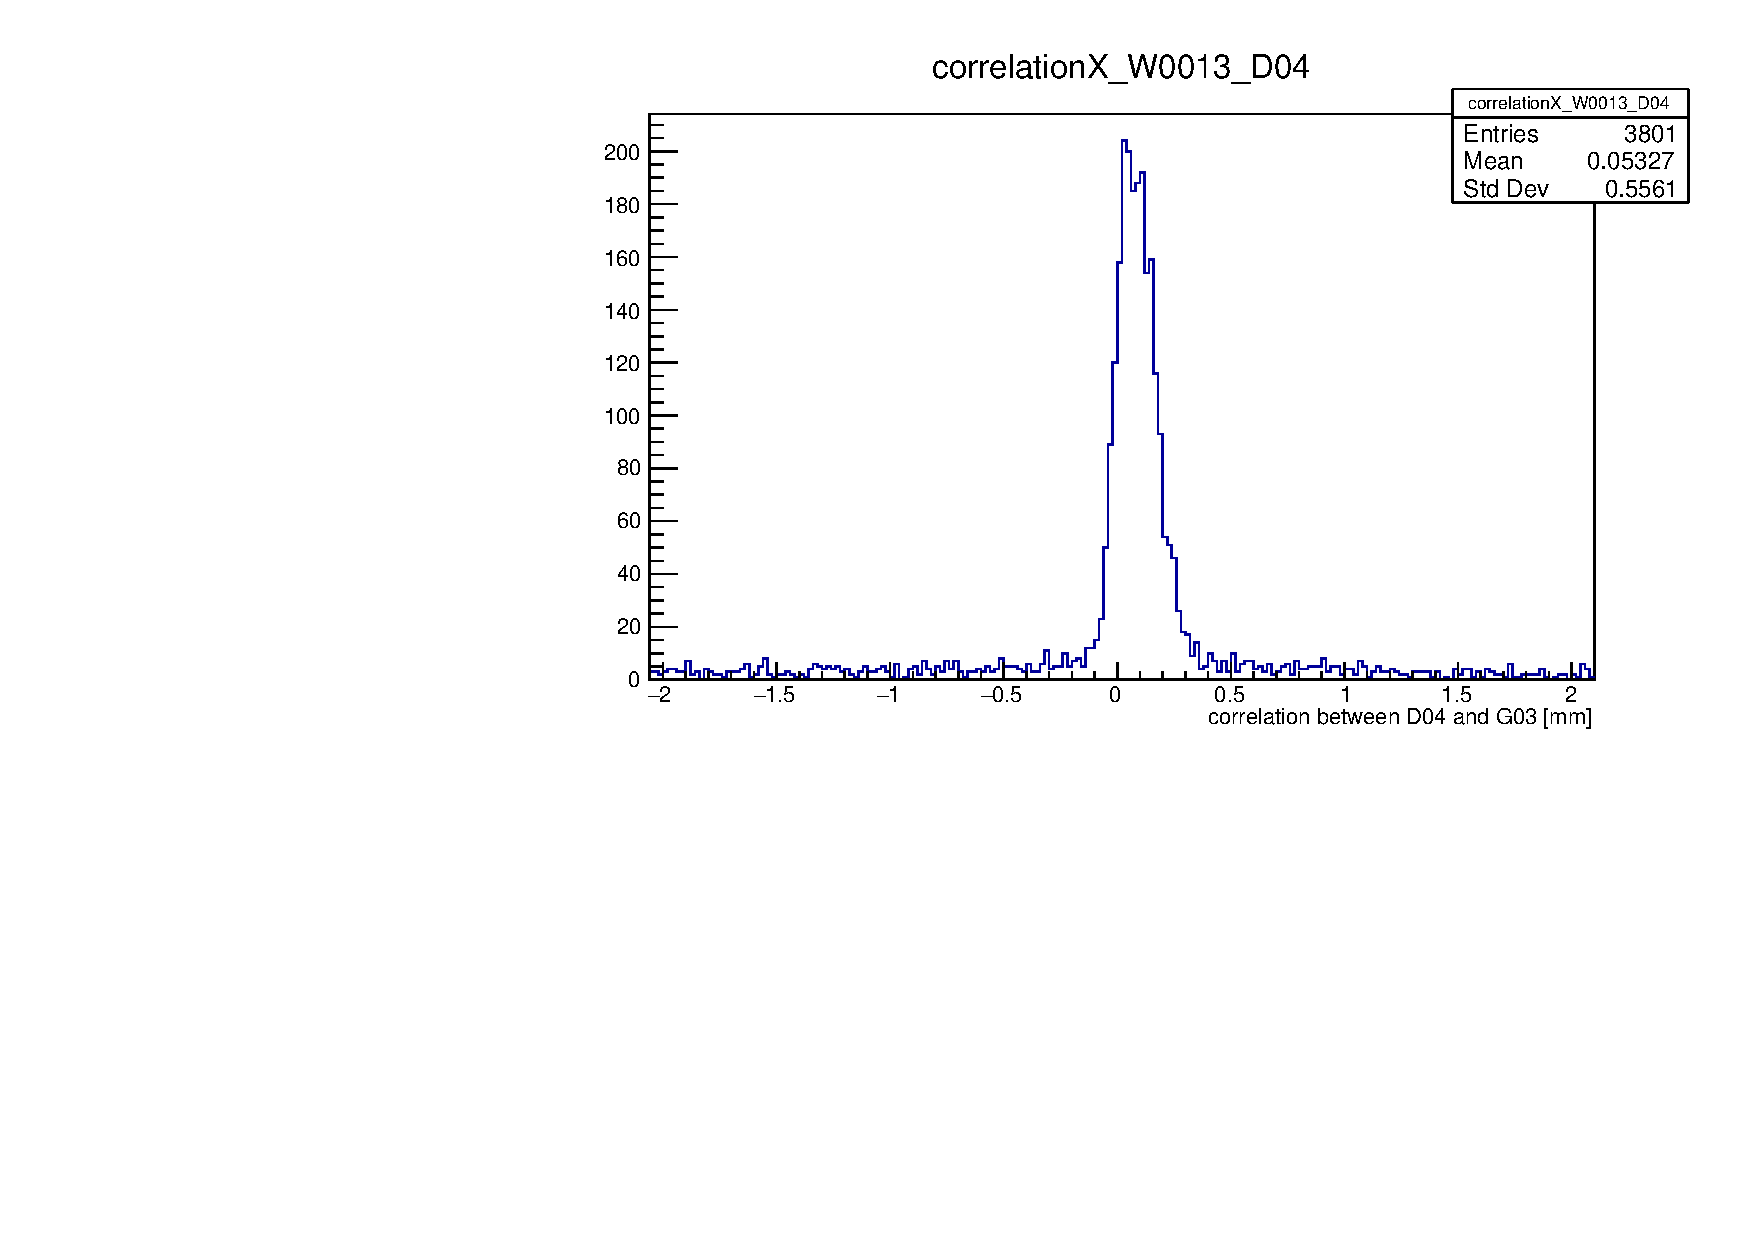
\includegraphics[width=\textwidth]{correlationX_D04_29519}
        \caption{Good example of a correlation plot.}
        \label{fig:correlationX}
    \end{subfigure}
    \begin{subfigure}[t]{0.66\textwidth}
        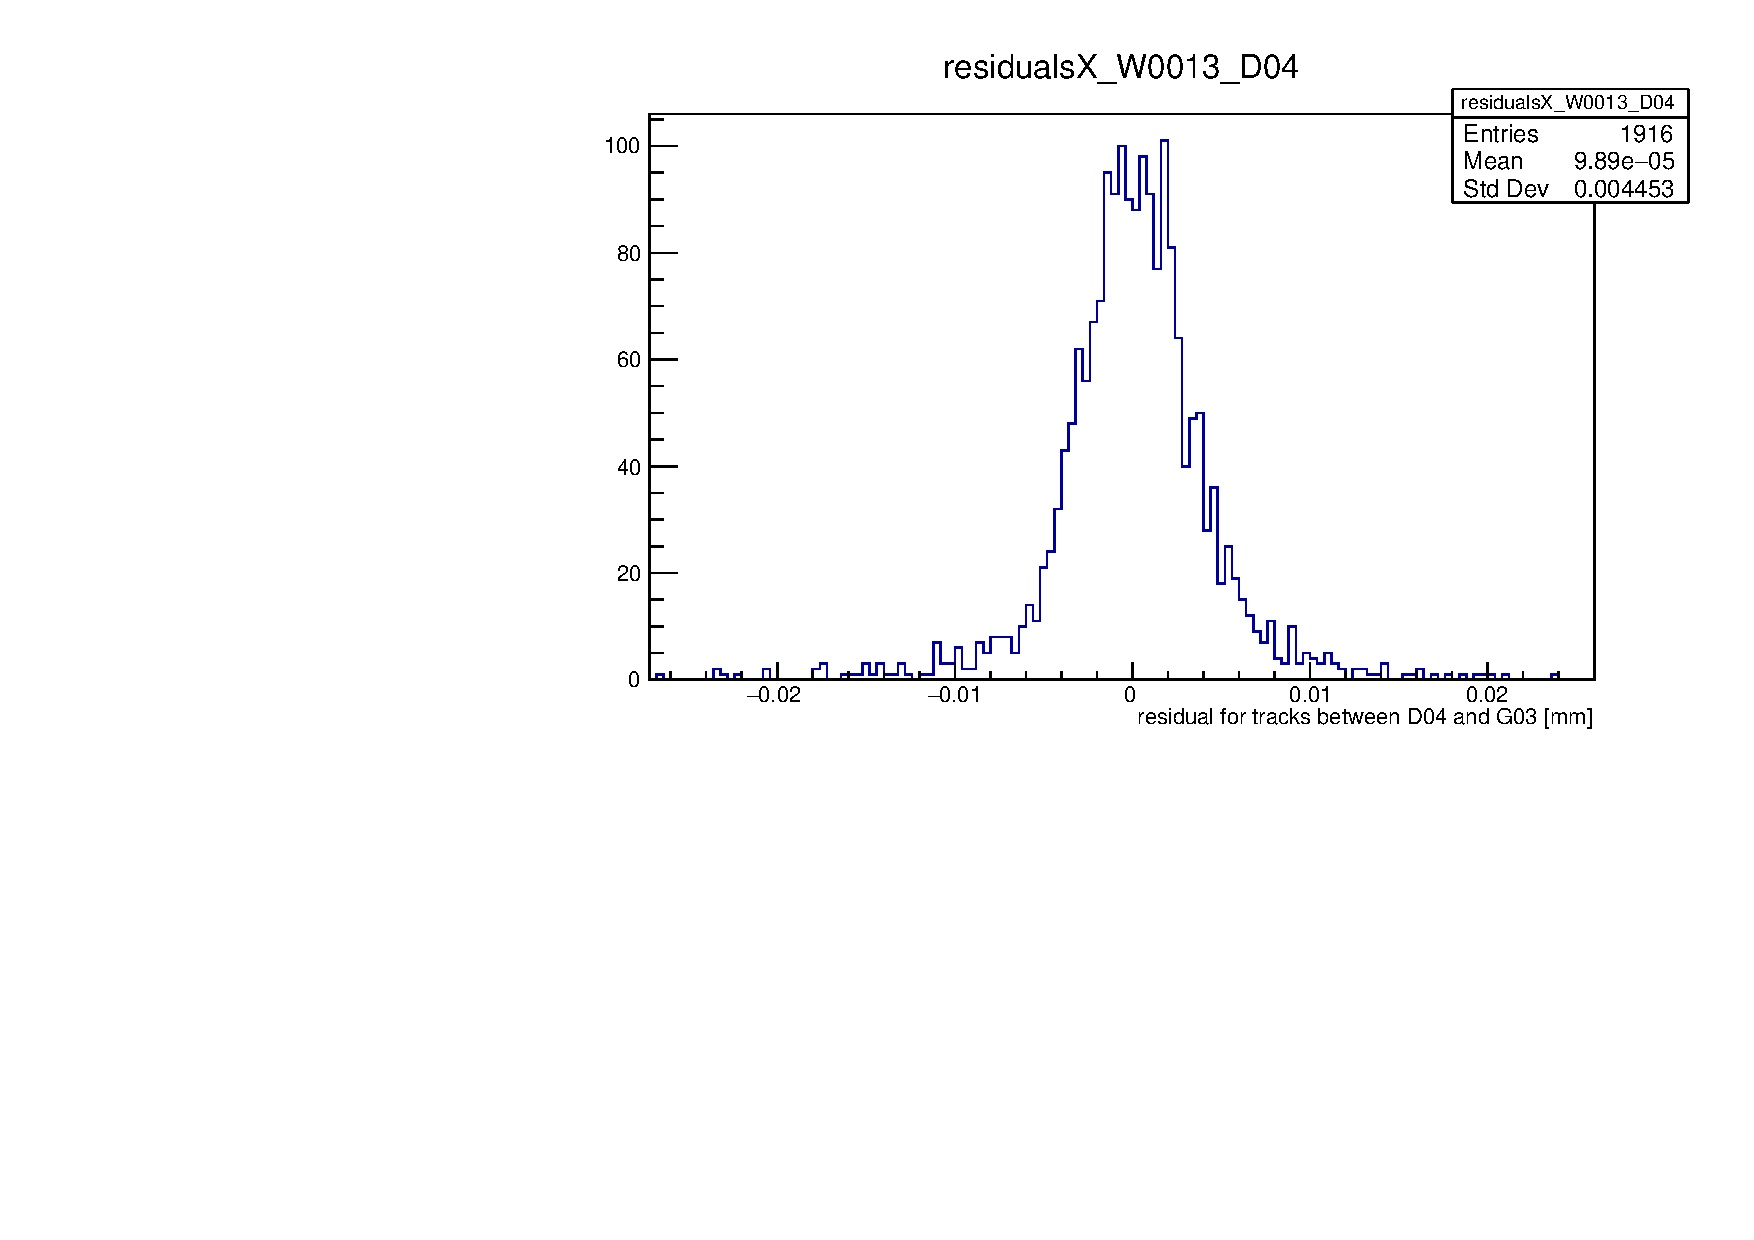
\includegraphics[width=\textwidth]{residualX_D04_29519}
        \caption{Good example of a residual distribution.}
        \label{fig:residualX}
    \end{subfigure}
    \caption{Examples of distributions as they should look like. \\ \textcolor{blue}{Jens: }\textcolor{orange}{Update with more statistics!}}
    \label{fig:exampleAlignment}
\end{figure}

\textbf{Note:} when re-running the procedure from a slightly different initial geometry, the resulting alignment (i.e.~the numbers in the detectors file) will differ slightly which is acceptable. What should \textbf{not} differ is the width of the residuals.

%\begin{figure}[h]
%	\centering
%	
\includegraphics[width=0.35\textwidth]{obama}
%	\caption{Placeholder}
%	\label{fig:placeholder}
%\end{figure}

\section{Aligning the DUT}
\label{sec:align_dut}
Once the telescope is aligned, its geometry is not touched anymore. From now on, it is used to build tracks which are then matched to clusters on the DUT.

\subsection*{Prealignment of the DUT}
The prealignment of the DUT follows the same strategy as for the telescope. To look at the current alignment, the script
\begin{verbatim}
    /path/to/corryvreckan/bin/corry 
    	-c analyse_atlaspix.conf 
    	-o detectors_file=<detectorsFile> 
    	-o histogramFile=<histogramFile> 
    	-o EventLoaderTimepix3.inputDirectory=<inputDir_TPX>
    	-o EventLoaderATLASpix.inputDirectory=<inputDir_APX>
\end{verbatim}
needs to be run.
If no better guess is available, the initial alignment of the DUT should be set to $x=y=z=0$.

Then, by repeatedly running \corry and modifying the position of the DUT in the detectors file one should be able to bring the peaks of the correlations in x and y close to 0.
If no peak at all can be seen in the correlation plots, check whether some values need to be corrected in the configuration file, most likely \texttt{clockCycle} or \texttt{clkdivend2} in \texttt{[EventLoaderATLASpix]}.

\textbf{Important: }If using the \texttt{[Prealignment]} module, make sure to add the \texttt{name} parameter.
Otherwise, the telescope planes are also shifted again destroying the telescope alignment.

\begin{minted}[frame=single,framesep=3pt,breaklines=true,tabsize=2,linenos]{ini}
...
[Prealignment]
name = "<DUT_name>"

[Ignore]
#[AlignmentDUTResiduals]
log_level=INFO
iterations = 4
alignOrientation=true
alignPosition=true
\end{minted}

\subsection*{Alignment of the DUT}
Again, the alignment strategy for the DUT is similar as for the telescope and requires multiple iterations.
In \texttt{align\_dut.conf}, check that the prealignment is disabled and the alignment is enabled.
Now, the algorithm optimizes the residuals of the tracks through the DUT:

\begin{minted}[frame=single,framesep=3pt,breaklines=true,tabsize=2,linenos]{ini}
...
#[Prealignment]
#[Ignore]
[AlignmentDUTResiduals]
log_level=INFO
iterations = 4
alignOrientation=true
alignPosition=true
\end{minted}

Then run
\begin{verbatim}
    /path/to/corryvreckan/bin/corry 
    	-c align_dut.conf 
    	-o detectors_file=<detectorsFile> 
    	-o detectors_file_updated=<detectorsFileUpdated> 
    	-o histogramFile=<histogramFile> 
    	-o EventLoaderTimepix3.inputDirectory=<inputDir_TPX>
    	-o EventLoaderATLASpix.inputDirectory=<inputDir_APX>
\end{verbatim}

\textbf{Note:} The histograms of the residuals for the DUT in \texttt{[Tracking4D]} are empty. The correct ones can be found in \texttt{[AnalysisDUT]}.

Like for the telescope alignment, the widths of the residuals can be interpreted as the spatial resolution of the DUT and should should thus be $\lesssim$~pixel size.
Again, starting with a \texttt{spatialCut} in \texttt{[DUTAssociation]} of multiple ($\sim4$) pixel sizes, it should be decreased incrementally down to the pixel size. Note that an asymmetric pixel geometry requires the \texttt{spatialCut} to be chosen accordingly.

If the alignment keeps to fail, it is possible to allow only for rotational or translational alignment while freezing the other for one or a few iterations.

\begin{minted}[frame=single,framesep=3pt,breaklines=true,tabsize=2,linenos]{ini}
...
#[Prealignment]
#[Ignore]
[AlignmentDUTResiduals]
log_level=INFO
iterations = 4
alignOrientation=false #<-- disable rotational alignment
alignPosition=true
\end{minted}

\section{FAQs and Special Remarks}
Here a bunch common problems and solutions are \textcolor{orange}{(will be)} listed.
\begin{itemize}
\item add any problem and/or solution here
\end{itemize}

\vspace{3cm}
\begin{figure}[h]
	\centering
	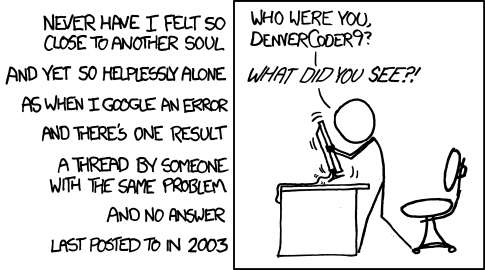
\includegraphics[width=0.66\textwidth]{wisdom_of_the_ancients}
	\caption{From \url{https://xkcd.com/979/}}
	\label{fig:wisdom}
\end{figure}
